% interactapasample.tex
% v1.05 - August 2017

\documentclass[]{interact}

\usepackage{epstopdf}% To incorporate .eps illustrations using PDFLaTeX, etc.
\usepackage[caption=false]{subfig}% Support for small, `sub' figures and tables
%\usepackage[nolists,tablesfirst]{endfloat}% To `separate' figures and tables from text if required
%\usepackage[doublespacing]{setspace}% To produce a `double spaced' document if required
%\setlength\parindent{24pt}% To increase paragraph indentation when line spacing is doubled

\usepackage[longnamesfirst,sort]{natbib}% Citation support using natbib.sty
\bibpunct[, ]{(}{)}{;}{a}{,}{,}% Citation support using natbib.sty
\renewcommand\bibfont{\fontsize{10}{12}\selectfont}% To set the list of references in 10 point font using natbib.sty

%\usepackage[natbibapa,nodoi]{apacite}% Citation support using apacite.sty. Commands using natbib.sty MUST be deactivated first!
%\setlength\bibhang{12pt}% To set the indentation in the list of references using apacite.sty. Commands using natbib.sty MUST be deactivated first!
%\renewcommand\bibliographytypesize{\fontsize{10}{12}\selectfont}% To set the list of references in 10 point font using apacite.sty. Commands using natbib.sty MUST be deactivated first!

\theoremstyle{plain}% Theorem-like structures provided by amsthm.sty
\newtheorem{theorem}{Theorem}[section]
\newtheorem{lemma}[theorem]{Lemma}
\newtheorem{corollary}[theorem]{Corollary}
\newtheorem{proposition}[theorem]{Proposition}

\theoremstyle{definition}
\newtheorem{definition}[theorem]{Definition}
\newtheorem{example}[theorem]{Example}

\theoremstyle{remark}
\newtheorem{remark}{Remark}
\newtheorem{notation}{Notation}

\begin{document}

\articletype{ARTICLE TEMPLATE}% Specify the article type or omit as appropriate

\title{Taylor \& Francis \LaTeX\ template for authors (\textsf{Interact} layout + American Psychological Association reference style)}

\author{
\name{A.~N. Author\textsuperscript{a}\thanks{CONTACT A.~N. Author. Email: latex.helpdesk@tandf.co.uk} and John Smith\textsuperscript{b}}
\affil{\textsuperscript{a}Taylor \& Francis, 4 Park Square, Milton Park, Abingdon, UK; \textsuperscript{b}Institut f\"{u}r Informatik, Albert-Ludwigs-Universit\"{a}t, Freiburg, Germany}
}

\maketitle

\begin{abstract}
This template is for authors who are preparing a manuscript for a Taylor \& Francis journal using the \LaTeX\ document preparation system and the \texttt{interact} class file, which is available via selected journals' home pages on the Taylor \& Francis website.
\end{abstract}

\begin{keywords}
Sections; lists; figures; tables; mathematics; fonts; references; appendices
\end{keywords}


\section{Introduction}

In order to assist authors in the process of preparing a manuscript for a journal, the Taylor \& Francis `\textsf{Interact}' layout style has been implemented as a \LaTeXe\ class file based on the \texttt{article} document class. A sample bibliography is also provided in order to assist with the formatting of your references.

Commands that differ from or are provided in addition to standard \LaTeXe\ are described in this document, which is \emph{not} a substitute for a \LaTeXe\ tutorial.

The \texttt{interactapasample.tex} file can be used as a template for a manuscript by cutting, pasting, inserting and deleting text as appropriate, using the preamble and the \LaTeX\ environments provided (e.g.\ \verb"\begin{abstract}", \verb"\begin{keywords}").


\subsection{The \textsf{Interact} class file}\label{class}

The \texttt{interact} class file preserves the standard \LaTeXe\ interface such that any document that can be produced using \texttt{article.cls} can also be produced with minimal alteration using the \texttt{interact} class file as described in this document.

If your article is accepted for publication it will be typeset as the journal requires in Minion Pro and/or Myriad Pro. Since most authors will not have these fonts installed, the page make-up is liable to alter slightly with the change of font. Also, the \texttt{interact} class file produces only single-column format, which is preferred for peer review and will be converted to two-column format by the typesetter if necessary during preparation of the proofs. Please therefore do not try to match the typeset format exactly, but use the standard \LaTeX\ fonts instead and ignore details such as slightly long lines of text or figures/tables not appearing in exact synchronization with their citations in the text: these details will be dealt with by the typesetter. Similarly, it is unnecessary to spend time addressing warnings in the log file -- if your .tex file compiles to produce a PDF document that correctly shows how you wish your paper to appear, such warnings will not prevent your source files being imported into the typesetter's program.


\subsection{Submission of manuscripts prepared using \emph{\LaTeX}}

Manuscripts for possible publication should be submitted to the Editors for review as directed in the journal's Instructions for Authors, and in accordance with any technical instructions provided in the journal's ScholarOne Manuscripts or Editorial Manager site. Your \LaTeX\ source file(s), the class file and any graphics files will be required in addition to the final PDF version when final, revised versions of accepted manuscripts are submitted.

Please ensure that any author-defined macros used in your article are gathered together in the preamble of your .tex file, i.e.\ before the \verb"\begin{document}" command. Note that if serious problems are encountered in the coding of a document (missing author-defined macros, for example), the typesetter may resort to rekeying it.


\section{Using the \texttt{interact} class file}

For convenience, simply copy the \texttt{interact.cls} file into the same directory as your manuscript files (you do not need to install it in your \TeX\ distribution). In order to use the \texttt{interact} document class, replace the command \verb"\documentclass{article}" at the beginning of your document with the command \verb"\documentclass{interact}".

The following document-class options should \emph{not} be used with the \texttt{interact} class file:
\begin{itemize}
  \item \texttt{10pt}, \texttt{11pt}, \texttt{12pt} -- unavailable;
  \item \texttt{oneside}, \texttt{twoside} -- not necessary, \texttt{oneside} is the default;
  \item \texttt{leqno}, \texttt{titlepage} -- should not be used;
  \item \texttt{twocolumn} -- should not be used (see Subsection~\ref{class});
  \item \texttt{onecolumn} -- not necessary as it is the default style.
\end{itemize}
To prepare a manuscript for a journal that is printed in A4 (two column) format, use the \verb"largeformat" document-class option provided by \texttt{interact.cls}; otherwise the class file produces pages sized for B5 (single column) format by default. The \texttt{geometry} package should not be used to make any further adjustments to the page dimensions.

%If your manuscript has supplementary content you can also use the \verb"interact" class file to prepare all or part of it using the \verb"suppldata" document-class option, which will suppress the `article history' date. This option \emph{must not} be used on any primary content. Note that authors are solely responsible for the preparation of all supplemental material.


\section{Additional features of the \texttt{interact} class file}

\subsection{Title, authors' names and affiliations, abstracts and article types}

The title should be generated at the beginning of your article using the \verb"\maketitle" command.
In the final version the author name(s) and affiliation(s) must be followed immediately by \verb"\maketitle" as shown below in order for them to be displayed in your PDF document.
To prepare an anonymous version for double-blind peer review, you can put the \verb"\maketitle" between the \verb"\title" and the \verb"\author" in order to hide the author name(s) and affiliation(s) temporarily.
Next you should include the abstract if your article has one, enclosed within an \texttt{abstract} environment.
The \verb"\articletype" command is also provided as an \emph{optional} element which should \emph{only} be included if your article actually needs it.
For example, the titles for this document begin as follows:
\begin{verbatim}
\articletype{ARTICLE TEMPLATE}

\title{Taylor \& Francis \LaTeX\ template for authors (\textsf{Interact}
layout + American Psychological Association reference style)}

\author{
\name{A.~N. Author\textsuperscript{a}\thanks{CONTACT A.~N. Author.
Email: latex.helpdesk@tandf.co.uk} and John Smith\textsuperscript{b}}
\affil{\textsuperscript{a}Taylor \& Francis, 4 Park Square, Milton
Park, Abingdon, UK; \textsuperscript{b}Institut f\"{u}r Informatik,
Albert-Ludwigs-Universit\"{a}t, Freiburg, Germany} }

\maketitle

\begin{abstract}
This template is for authors who are preparing a manuscript for a
Taylor \& Francis journal using the \LaTeX\ document preparation system
and the \texttt{interact} class file, which is available via selected
journals' home pages on the Taylor \& Francis website.
\end{abstract}
\end{verbatim}

An additional abstract in another language (preceded by a translation of the article title) may be included within the \verb"abstract" environment if required.

A graphical abstract may also be included if required. Within the \verb"abstract" environment you can include the code
\begin{verbatim}
\\\resizebox{25pc}{!}{\includegraphics{abstract.eps}}
\end{verbatim}
where the graphical abstract is to appear, where \verb"abstract.eps" is the name of the file containing the graphic (note that \verb"25pc" is the recommended maximum width, expressed in pica, for the graphical abstract in your manuscript).


\subsection{Abbreviations}

A list of abbreviations may be included if required, enclosed within an \texttt{abbreviations} environment, i.e.\ \verb"\begin{abbreviations}"\ldots\verb"\end{abbreviations}", immediately following the \verb"abstract" environment.


\subsection{Keywords}

A list of keywords may be included if required, enclosed within a \texttt{keywords} environment, i.e.\ \verb"\begin{keywords}"\ldots\verb"\end{keywords}". Additional keywords in other languages (preceded by a translation of the word `keywords') may also be included within the \verb"keywords" environment if required.


\subsection{Subject classification codes}

AMS, JEL or PACS classification codes may be included if required. The \texttt{interact} class file provides an \texttt{amscode} environment, i.e.\ \verb"\begin{amscode}"\ldots\verb"\end{amscode}", a \texttt{jelcode} environment, i.e.\ \verb"\begin{jelcode}"\ldots\verb"\end{jelcode}", and a \texttt{pacscode} environment, i.e.\ \verb"\begin{pacscode}"\ldots\verb"\end{pacscode}" to assist with this.


\subsection{Additional footnotes to the title or authors' names}

The \verb"\thanks" command may be used to create additional footnotes to the title or authors' names if required. Footnote symbols for this purpose should be used in the order
$^\ast$~(coded as \verb"$^\ast$"), $\dagger$~(\verb"$\dagger$"), $\ddagger$~(\verb"$\ddagger$"), $\S$~(\verb"$\S$"), $\P$~(\verb"$\P$"), $\|$~(\verb"$\|$"),
$\dagger\dagger$~(\verb"$\dagger\dagger$"), $\ddagger\ddagger$~(\verb"$\ddagger\ddagger$"), $\S\S$~(\verb"$\S\S$"), $\P\P$~(\verb"$\P\P$").

Note that any \verb"footnote"s to the main text will automatically be assigned the superscript symbols 1, 2, 3, etc. by the class file.\footnote{If preferred, the \texttt{endnotes} package may be used to set the notes at the end of your text, before the bibliography. The symbols will be changed to match the style of the journal if necessary by the typesetter.}


\section{Some guidelines for using the standard features of \LaTeX}

\subsection{Sections}

The \textsf{Interact} layout style allows for five levels of section heading, all of which are provided in the \texttt{interact} class file using the standard \LaTeX\ commands \verb"\section", \verb"\subsection", \verb"\subsubsection", \verb"\paragraph" and \verb"\subparagraph". Numbering will be automatically generated for all these headings by default.


\subsection{Lists}

Numbered lists are produced using the \texttt{enumerate} environment, which will number each list item with arabic numerals by default. For example,
\begin{enumerate}
  \item first item
  \item second item
  \item third item
\end{enumerate}
was produced by
\begin{verbatim}
\begin{enumerate}
  \item first item
  \item second item
  \item third item
\end{enumerate}
\end{verbatim}
Alternative numbering styles can be achieved by inserting an optional argument in square brackets to each \verb"item", e.g.\ \verb"\item[(i)] first item"\, to create a list numbered with roman numerals at level one.

Bulleted lists are produced using the \texttt{itemize} environment. For example,
\begin{itemize}
  \item First bulleted item
  \item Second bulleted item
  \item Third bulleted item
\end{itemize}
was produced by
\begin{verbatim}
\begin{itemize}
  \item First bulleted item
  \item Second bulleted item
  \item Third bulleted item
\end{itemize}
\end{verbatim}


\subsection{Figures}

The \texttt{interact} class file will deal with positioning your figures in the same way as standard \LaTeX. It should not normally be necessary to use the optional \texttt{[htb]} location specifiers of the \texttt{figure} environment in your manuscript; you may, however, find the \verb"[p]" placement option or the \verb"endfloat" package useful if a journal insists on the need to separate figures from the text.

Figure captions appear below the figures themselves, therefore the \verb"\caption" command should appear after the body of the figure. For example, Figure~\ref{sample-figure} with caption and sub-captions is produced using the following commands:
\begin{verbatim}
\begin{figure}
\centering
\subfloat[An example of an individual figure sub-caption.]{%
\resizebox*{5cm}{!}{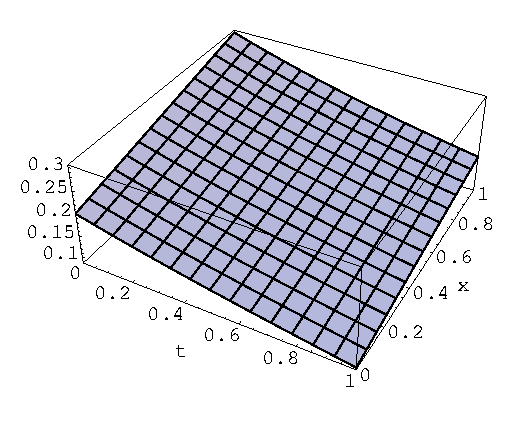
\includegraphics{graph1.eps}}}\hspace{5pt}
\subfloat[A slightly shorter sub-caption.]{%
\resizebox*{5cm}{!}{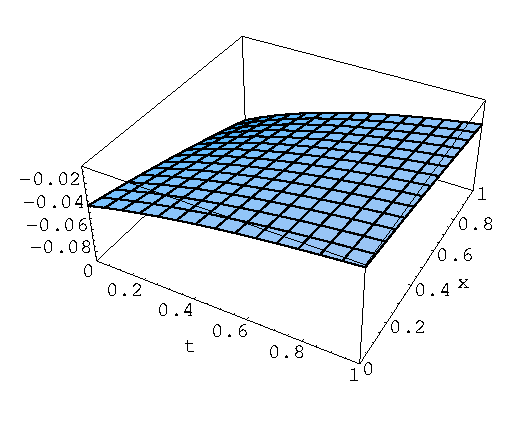
\includegraphics{graph2.eps}}}
\caption{Example of a two-part figure with individual sub-captions
 showing that captions are flush left and justified if greater
 than one line of text.} \label{sample-figure}
\end{figure}
\end{verbatim}
\begin{figure}
\centering
\subfloat[An example of an individual figure sub-caption.]{%
\resizebox*{5cm}{!}{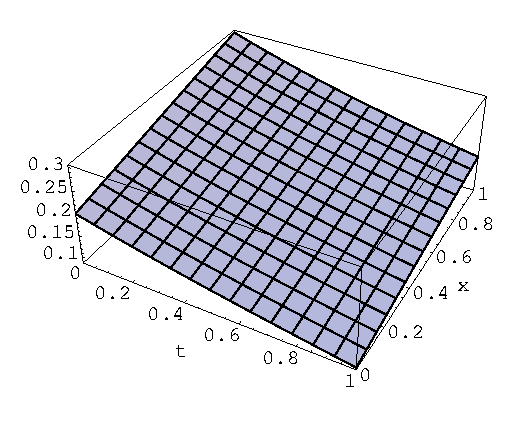
\includegraphics{graph1.eps}}}\hspace{5pt}
\subfloat[A slightly shorter sub-caption.]{%
\resizebox*{5cm}{!}{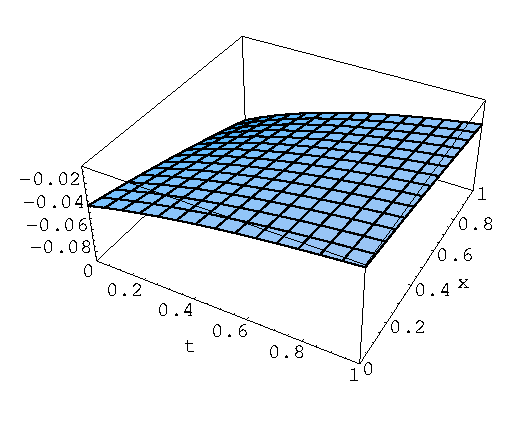
\includegraphics{graph2.eps}}}
\caption{Example of a two-part figure with individual sub-captions
 showing that captions are flush left and justified if greater
 than one line of text.} \label{sample-figure}
\end{figure}

To ensure that figures are correctly numbered automatically, the \verb"\label" command should be included just after the \verb"\caption" command, or in its argument.

The \verb"\subfloat" command requires \verb"subfig.sty", which is called in the preamble of the \texttt{interactapasample.tex} file (to allow your choice of an alternative package if preferred) and included in the \textsf{Interact} \LaTeX\ bundle for convenience. Please supply any additional figure macros used with your article in the preamble of your .tex file.

The source files of any figures will be required when the final, revised version of a manuscript is submitted. Authors should ensure that these are suitable (in terms of lettering size, etc.) for the reductions they envisage.

The \texttt{epstopdf} package can be used to incorporate encapsulated PostScript (.eps) illustrations when using PDF\LaTeX, etc. Please provide the original .eps source files rather than the generated PDF images of those illustrations for production purposes.


\subsection{Tables}

The \texttt{interact} class file will deal with positioning your tables in the same way as standard \LaTeX. It should not normally be necessary to use the optional \texttt{[htb]} location specifiers of the \texttt{table} environment in your manuscript; you may, however, find the \verb"[p]" placement option or the \verb"endfloat" package useful if a journal insists on the need to separate tables from the text.

The \texttt{tabular} environment can be used as shown to create tables with single horizontal rules at the head, foot and elsewhere as appropriate. The captions appear above the tables in the \textsf{Interact} style, therefore the \verb"\tbl" command should be used before the body of the table. For example, Table~\ref{sample-table} is produced using the following commands:
\begin{table}
\tbl{Example of a table showing that its caption is as wide as
 the table itself and justified.}
{\begin{tabular}{lcccccc} \toprule
 & \multicolumn{2}{l}{Type} \\ \cmidrule{2-7}
 Class & One & Two & Three & Four & Five & Six \\ \midrule
 Alpha\textsuperscript{a} & A1 & A2 & A3 & A4 & A5 & A6 \\
 Beta & B2 & B2 & B3 & B4 & B5 & B6 \\
 Gamma & C2 & C2 & C3 & C4 & C5 & C6 \\ \bottomrule
\end{tabular}}
\tabnote{\textsuperscript{a}This footnote shows how to include
 footnotes to a table if required.}
\label{sample-table}
\end{table}
\begin{verbatim}
\begin{table}
\tbl{Example of a table showing that its caption is as wide as
 the table itself and justified.}
{\begin{tabular}{lcccccc} \toprule
 & \multicolumn{2}{l}{Type} \\ \cmidrule{2-7}
 Class & One & Two & Three & Four & Five & Six \\ \midrule
 Alpha\textsuperscript{a} & A1 & A2 & A3 & A4 & A5 & A6 \\
 Beta & B2 & B2 & B3 & B4 & B5 & B6 \\
 Gamma & C2 & C2 & C3 & C4 & C5 & C6 \\ \bottomrule
\end{tabular}}
\tabnote{\textsuperscript{a}This footnote shows how to include
 footnotes to a table if required.}
\label{sample-table}
\end{table}
\end{verbatim}

To ensure that tables are correctly numbered automatically, the \verb"\label" command should be included just before \verb"\end{table}".

The \verb"\toprule", \verb"\midrule", \verb"\bottomrule" and \verb"\cmidrule" commands are those used by \verb"booktabs.sty", which is called by the \texttt{interact} class file and included in the \textsf{Interact} \LaTeX\ bundle for convenience. Tables produced using the standard commands of the \texttt{tabular} environment are also compatible with the \texttt{interact} class file.


\subsection{Landscape pages}

If a figure or table is too wide to fit the page it will need to be rotated, along with its caption, through 90$^{\circ}$ anticlockwise. Landscape figures and tables can be produced using the \verb"rotating" package, which is called by the \texttt{interact} class file. The following commands (for example) can be used to produce such pages.
\begin{verbatim}
\setcounter{figure}{1}
\begin{sidewaysfigure}
\centerline{\epsfbox{figname.eps}}
\caption{Example landscape figure caption.}
\label{landfig}
\end{sidewaysfigure}
\end{verbatim}
\begin{verbatim}
\setcounter{table}{1}
\begin{sidewaystable}
 \tbl{Example landscape table caption.}
  {\begin{tabular}{@{}llllcll}
    .
    .
    .
  \end{tabular}}\label{landtab}
\end{sidewaystable}
\end{verbatim}
Before any such float environment, use the \verb"\setcounter" command as above to fix the numbering of the caption (the value of the counter being the number given to the preceding figure or table). Subsequent captions will then be automatically renumbered accordingly. The \verb"\epsfbox" command requires \verb"epsfig.sty", which is called by the \texttt{interact} class file and is also included in the \textsf{Interact} \LaTeX\ bundle for convenience.

Note that if the \verb"endfloat" package is used, one or both of the commands
\begin{verbatim}
\DeclareDelayedFloatFlavor{sidewaysfigure}{figure}
\DeclareDelayedFloatFlavor{sidewaystable}{table}
\end{verbatim}
will need to be included in the preamble of your .tex file, after the \verb"endfloat" package is loaded, in order to process any landscape figures and/or tables correctly.


\subsection{Theorem-like structures}

A predefined \verb"proof" environment is provided by the \texttt{amsthm} package (which is called by the \texttt{interact} class file), as follows:
\begin{proof}
More recent algorithms for solving the semidefinite programming relaxation are particularly efficient, because they explore the structure of the MAX-CUT problem.
\end{proof}
\noindent This was produced by simply typing:
\begin{verbatim}
\begin{proof}
More recent algorithms for solving the semidefinite programming
relaxation are particularly efficient, because they explore the
structure of the MAX-CUT problem.
\end{proof}
\end{verbatim}
Other theorem-like environments (theorem, definition, remark, etc.) need to be defined as required, e.g.\ using \verb"\newtheorem{theorem}{Theorem}" in the preamble of your .tex file (see the preamble of \verb"interactapasample.tex" for more examples). You can define the numbering scheme for these structures however suits your article best. Please note that the format of the text in these environments may be changed if necessary to match the style of individual journals by the typesetter during preparation of the proofs.


\subsection{Mathematics}

\subsubsection{Displayed mathematics}

The \texttt{interact} class file will set displayed mathematical formulas centred on the page without equation numbers if you use the \texttt{displaymath} environment or the equivalent \verb"\[...\]" construction. For example, the equation
\[
 \hat{\theta}_{w_i} = \hat{\theta}(s(t,\mathcal{U}_{w_i}))
\]
was typeset using the commands
\begin{verbatim}
\[
 \hat{\theta}_{w_i} = \hat{\theta}(s(t,\mathcal{U}_{w_i}))
\]
\end{verbatim}

For those of your equations that you wish to be automatically numbered sequentially throughout the text for future reference, use the \texttt{equation} environment, e.g.
\begin{equation}
 \hat{\theta}_{w_i} = \hat{\theta}(s(t,\mathcal{U}_{w_i}))
\end{equation}
was typeset using the commands
\begin{verbatim}
\begin{equation}
 \hat{\theta}_{w_i} = \hat{\theta}(s(t,\mathcal{U}_{w_i}))
\end{equation}
\end{verbatim}

Part numbers for sets of equations may be generated using the \texttt{subequations} environment, e.g.
\begin{subequations} \label{subeqnexample}
\begin{equation}
     \varepsilon \rho w_{tt}(s,t) = N[w_{s}(s,t),w_{st}(s,t)]_{s},
     \label{subeqnparta}
\end{equation}
\begin{equation}
     w_{tt}(1,t)+N[w_{s}(1,t),w_{st}(1,t)] = 0,   \label{subeqnpartb}
\end{equation}
\end{subequations}
which was typeset using the commands
\begin{verbatim}
\begin{subequations} \label{subeqnexample}
\begin{equation}
     \varepsilon \rho w_{tt}(s,t) = N[w_{s}(s,t),w_{st}(s,t)]_{s},
     \label{subeqnparta}
\end{equation}
\begin{equation}
     w_{tt}(1,t)+N[w_{s}(1,t),w_{st}(1,t)] = 0,   \label{subeqnpartb}
\end{equation}
\end{subequations}
\end{verbatim}
This is made possible by the \texttt{amsmath} package, which is called by the class file. If you put a \verb"\label" just after the \verb"\begin{subequations}" command, references can be made to the collection of equations, i.e.\ `(\ref{subeqnexample})' in the example above. Or, as the example also shows, you can label and refer to each equation individually -- i.e.\ `(\ref{subeqnparta})' and `(\ref{subeqnpartb})'.

Displayed mathematics should be given end-of-line punctuation appropriate to the running text sentence of which it forms a part, if required.

\subsubsection{Math fonts}

\paragraph{Superscripts and subscripts}
Superscripts and subscripts will automatically come out in the correct size in a math environment (i.e.\ enclosed within \verb"\(...\)" or \verb"$...$" commands in running text, or within \verb"\[...\]" or the \texttt{equation} environment for displayed equations). Sub/superscripts that are physical variables should be italic, whereas those that are labels should be roman (e.g.\ $C_p$, $T_\mathrm{eff}$). If the subscripts or superscripts need to be other than italic, they must be coded individually.

\paragraph{Upright Greek characters and the upright partial derivative sign}
Upright lowercase Greek characters can be obtained by inserting the letter `u' in the control code for the character, e.g.\ \verb"\umu" and \verb"\upi" produce $\umu$ (used, for example, in the symbol for the unit microns -- $\umu\mathrm{m}$) and $\upi$ (the ratio of the circumference of a circle to its diameter). Similarly, the control code for the upright partial derivative $\upartial$ is \verb"\upartial". Bold lowercase as well as uppercase Greek characters can be obtained by \verb"{\bm \gamma}", for example, which gives ${\bm \gamma}$, and \verb"{\bm \Gamma}", which gives ${\bm \Gamma}$.


\section*{Acknowledgement(s)}

An unnumbered section, e.g.\ \verb"\section*{Acknowledgements}", may be used for thanks, etc.\ if required and included \emph{in the non-anonymous version} before any Notes or References.


\section*{Disclosure statement}

An unnumbered section, e.g.\ \verb"\section*{Disclosure statement}", may be used to declare any potential conflict of interest and included \emph{in the non-anonymous version} before any Notes or References, after any Acknowledgements and before any Funding information.


\section*{Funding}

An unnumbered section, e.g.\ \verb"\section*{Funding}", may be used for grant details, etc.\ if required and included \emph{in the non-anonymous version} before any Notes or References.


\section*{Notes on contributor(s)}

An unnumbered section, e.g.\ \verb"\section*{Notes on contributors}", may be included \emph{in the non-anonymous version} if required. A photograph may be added if requested.


\section*{Nomenclature/Notation}

An unnumbered section, e.g.\ \verb"\section*{Nomenclature}" (or \verb"\section*{Notation}"), may be included if required, before any Notes or References.


\section*{Notes}

An unnumbered `Notes' section may be included before the References (if using the \verb"endnotes" package, use the command \verb"\theendnotes" where the notes are to appear, instead of creating a \verb"\section*").


\section{References}

\subsection{References cited in the text}

References should be cited in accordance with \citeauthor{APA10} (APA) style, i.e.\ in alphabetical order separated by semicolons, e.g.\ `\citep{Ban77,Pia88,VL07}' or `\ldots see Smith (1985, p.~75)'. If there are two or more authors with the same surname, use the first author's initials with the surnames, e.g.\ `\citep{Lig08,Lig06}'. If there are three to five authors, list all the authors in the first citation, e.g.\ `\citep{GSSM91}'. In subsequent citations, use only the first author's surname followed by et al., e.g.\ `\citep{GSSM91}'. For six or more authors, cite the first author's name followed by et al. For two or more sources by the same author(s) in the same year, use lower-case letters (a,~b,~c, \ldots) with the year to order the entries in the reference list and use these lower-case letters with the year in the in-text citations, e.g.\ `(Green, 1981a,b)'. For further details on this reference style, see the Instructions for Authors on the Taylor \& Francis website.

Each bibliographic entry has a key, which is assigned by the author and is used to refer to that entry in the text. In this document, the key \verb"Nas93" in the citation form \verb"\citep{Nas93}" produces `\citep{Nas93}', and the keys \verb"Koc59", \verb"Han04" and \verb"Cla08" in the citation form \verb"\citep{Koc59,Han04,Cla08}" produce `\citep{Koc59,Han04,Cla08}'. The citation \verb"\citep{Cha08}" produces `\citep{Cha08}' where the citation first appears in the text, and `\citep{Cha08}' in any subsequent citation. The appropriate citation style for different situations can be obtained, for example, by \verb"\citet{Ovi95}" for `\citet{Ovi95}', \verb"\citealp{MPW08}" for `\citealp{MPW08}', and \verb"\citealt{Sch93}" for `\citealt{Sch93}'. Citation of the year alone may be produced by \verb"\citeyear{Sch00}", i.e.\ `\citeyear{Sch00}', or \verb"\citeyearpar{Gra05}", i.e.\ `\citeyearpar{Gra05}', or of the author(s) alone by \verb"\citeauthor{Rit74}", i.e.\ `\citeauthor{Rit74}'. Optional notes may be included at the beginning and/or end of a citation by the use of square brackets, e.g.\ \verb"\citep[p.~31]{Hay08}" produces `\citep[p.~31]{Hay08}'; \verb"\citep[see][pp.~73-–77]{PI51}" produces `\citep[see][pp.~73--77]{PI51}'; \verb"\citep[e.g.][]{Fel81}" produces `\citep[e.g.][]{Fel81}'. A `plain' \verb"\cite" command will produce the same results as a \verb"\citet", i.e.\ \verb"\cite{BriIP}" will produce `\cite{BriIP}'.


\subsection{The list of references}

References should be listed at the end of the main text in alphabetical order, then chronologically (earliest first), with full page ranges (where appropriate) and issue numbers (essential for journals paginated by issue). If a reference has more than seven named authors, list the first six names, followed by an ellipsis (\ldots), then the last author's name \cite[see for example][]{Gil04}.
The following list shows some sample references prepared in the Taylor \& Francis APA style.

\begin{thebibliography}{}

\bibitem[American Psychological Association(2010)]{APA10}
American Psychological Association. (2010). \emph {Publication manual of the
 American Psychological Association} (6th ed.). Washington, DC: Author.

\bibitem[Bandura(1977)]{Ban77}
Bandura, A.~J. (1977). \emph{Social learning theory}. Englewood Cliffs, NJ:
 Prentice Hall.

\bibitem[Briscoe(in press)]{BriIP}
Briscoe, R. (in press). {Egocentric spatial representation in action and
 perception}. \emph{Philosophy and Phenomenological Research}. Retrieved from
 http://cogprints.org/5780/1/ECSRAP.F07.pdf

\bibitem[Chamberlin et al.(2008)Chamberlin, Novotney, Packard, \& Price]{Cha08}
Chamberlin, J., Novotney, A., Packard, E., \& Price, M. (2008, May).
 Enhancing worker well-being: Occupational health psychologists convene to
 share their research on work, stress, and health. \emph{Monitor on
 Psychology}, \emph{39}(5), 26--29.

\bibitem[Clay(2008)]{Cla08}
Clay, R. (2008, June). Science vs. ideology: Psychologists fight back about the
 misuse of research. \emph{Monitor on Psychology}, \emph{39}(6). Retrieved from
 http://www.apa.org/monitor/

\bibitem[Feller(1981)]{Fel81}
Feller, B.~A. (1981). \emph{Health characteristics of persons with chronic
 activity limitation, United States, 1979} (Report No. VHS-SER10/137).
 Hyattsville, MD: National Center for Health Statistics (US).

\bibitem[Ganster et~al.(1991)Ganster, Schaubroeck, Sime, \& Mayes]{GSSM91}
Ganster, D.~C., Schaubroeck, J., Sime, W.~E., \& Mayes, B.~T. (1991).
 The nomological validity of the Type A personality among employed adults
 [Monograph]. \emph{Journal of Applied Psychology}, \emph{76}, 143--168.

\bibitem[Gilbert et~al.(2004)]{Gil04}
Gilbert, D.~G., McClernon, F.~J., Rabinovich, N.~E., Sugai, C., Plath, L.~C.,
 Asgaard, G., \ldots Botros, N. (2004). Effects of quitting smoking on EEG
 activation and attention last for more than 31 days and are more severe with
 stress, dependence, DRD2 A1 allele, and depressive traits. \emph{Nicotine
 and Tobacco Research}, \emph{6}, 249--267.

\bibitem[Graham(2005)]{Gra05}
Graham, G. (2005). Behaviorism. In E.~N. Zalta (ed.), \emph{The Stanford
 encyclopedia of philosophy} (Fall 2007 ed.). Retrieved from
 http://plato.stanford.edu/entries/behaviorism

\bibitem[Haney \& Wiener(2004)]{Han04}
Haney, C., \& Wiener, R.~L. (Eds.). (2004). Capital punishment in the United
 States [Special issue]. \emph{Psychology, Public Policy, and Law},
 \emph{10}(4).

\bibitem[Haybron(2008)]{Hay08}
Haybron, D.~M. (2008). Philosophy and the science of subjective well-being. In
 M. Eid \& R.~J. Larsen (Eds.), \emph{The science of subjective well-being}
 (pp. 17--43). New York, NY: Guilford Press.

\bibitem[Koch(1959-1963)]{Koc59}
Koch, S. (Ed.). (1959--1963). \emph{Psychology: A study of science}
 (Vols.~1--6). New York, NY: McGraw-Hill.

\bibitem[I. Light(2006)]{Lig06}
Light, I. (2006). \emph{Deflecting immigration: Networks, markets, and
 regulation in Los Angeles}. New York, NY: Russell Sage Foundation.

\bibitem[M.~A. Light \& Light(2008)]{Lig08}
Light, M.~A., \& Light, I.~H. (2008). The geographic expansion of Mexican
 immigration in the United States and its applications for local law
 enforcement. \emph{Law Enforcement Executive Forum Journal}, \emph{8}(1),
 73--82.

\bibitem[Marshall-Pescini \& Whiten(2008)]{MPW08}
Marshall-Pescini, S., \& Whiten, A. (2008). Social learning of nut-cracking
 behavior in East African sanctuary-living chimpanzees (\emph{Pan troglodytes
 schweinfurthii}) [Supplemental material]. \emph{Journal of Comparative
 Psychology}, \emph{122}, 186--194.

\bibitem[Nash(1993)]{Nas93}
Nash, M. (1993). Malay. In P.~Hockings (Ed.), \emph{Encyclopedia of world
 cultures} (Vol.~5, pp.~174--176). New York, NY: G.~K. Hall.

\bibitem[Oviedo(1995)]{Ovi95}
Oviedo, S. (1995). \emph{Adolescent pregnancy: Voices heard in the everyday
 lives of pregnant teenagers} (Unpublished master's thesis). University of
 North Texas, Denton, TX.

\bibitem[Piaget(1988)]{Pia88}
Piaget, J. (1988). Extracts from Piaget's theory (G.~Gellerier \& J.~Langer,
 Trans.). In K.~Richardson \& S.~Sheldon (Eds.), \emph{Cognitive development
 to adolescence: A reader} (pp. 3--18). Hillsdale, NJ: Erlbaum. (Reprinted
 from \emph{Manual of child psychology}, pp. 703--732, by P.~H. Mussen, Ed.,
 1970, New York, NY: Wiley)

\bibitem[Piaget \& Inhelder(1951)]{PI51}
Piaget, J., \& Inhelder, B. (1951). \emph{La gen{\`e}se de l'id{\'e}e de
 hasard chez l'enfant} [The origin of the idea of chance in the child]. Paris:
 Presses Universitaires de France.

\bibitem[Ritzmann(1974)]{Rit74}
Ritzmann, R.~E. (1974). \emph{The snapping mechanism of \emph{Alpheid} shrimp}
 (Unpublished doctoral dissertation). University of Virginia, Charlottesville,
 VA.

\bibitem[Schatz(2000)]{Sch00}
Schatz, B.~R. (2000, November 17). Learning by text or context? [Review of the
 book \emph{The social life of information}, by J.~S. Brown \& P. Duguid].
\emph{Science}, \emph{290}, 1304.

\bibitem[Schwartz(1993)]{Sch93}
Schwartz, J. (1993, September 30). Obesity affects economic, social status.
 \emph{The Washington Post}, pp.~A1, A4.

\bibitem[Von~Ledebur(2007)]{VL07}
Von~Ledebur, S.~C. (2007). Optimizing knowledge transfer by new employees in
 companies. \emph{Knowledge Management Research \& Practice}. Advance online
 publication. doi:10.1057/palgrave/kmrp.8500141

\end{thebibliography}
\bigskip
\noindent This was produced by typing:
\begin{verbatim}
\begin{thebibliography}{}

\bibitem[American Psychological Association(2010)]{APA10}
American Psychological Association. (2010). \emph {Publication manual
 of the American Psychological Association} (6th ed.). Washington, DC:
 Author.

\bibitem[Bandura(1977)]{Ban77}
Bandura, A.~J. (1977). \emph{Social learning theory}. Englewood Cliffs,
 NJ: Prentice Hall.

\bibitem[Briscoe(in press)]{BriIP}
Briscoe, R. (in press). {Egocentric spatial representation in action
 and perception}. \emph{Philosophy and Phenomenological Research}.
 Retrieved from http://cogprints.org/5780/1/ECSRAP.F07.pdf

\bibitem[Chamberlin et al.(2008)Chamberlin, Novotney, Packard, \& Price]{Cha08}
Chamberlin, J., Novotney, A., Packard, E., \& Price, M. (2008, May).
 Enhancing worker well-being: Occupational health psychologists convene
 to share their research on work, stress, and health. \emph{Monitor on
 Psychology}, \emph{39}(5), 26--29.

\bibitem[Clay(2008)]{Cla08}
Clay, R. (2008, June). Science vs. ideology: Psychologists fight back
 about the misuse of research. \emph{Monitor on Psychology},
 \emph{39}(6). Retrieved from http://www.apa.org/monitor/

\bibitem[Feller(1981)]{Fel81}
Feller, B.~A. (1981). \emph{Health characteristics of persons with chronic
 activity limitation, United States, 1979} (Report No. VHS-SER10/137).
 Hyattsville, MD: National Center for Health Statistics (US).

\bibitem[Ganster et al.(1991)Ganster, Schaubroeck, Sime, \& Mayes]{GSSM91}
Ganster, D.~C., Schaubroeck, J., Sime, W.~E., \& Mayes, B.~T. (1991).
 The nomological validity of the Type A personality among employed
 adults [Monograph]. \emph{Journal of Applied Psychology}, \emph{76},
 143--168.

\bibitem[Gilbert et~al.(2004)]{Gil04}
Gilbert, D.~G., McClernon, F.~J., Rabinovich, N.~E., Sugai, C., Plath,
 L.~C., Asgaard, G., \ldots Botros, N. (2004). Effects of quitting
 smoking on EEG activation and attention last for more than 31 days and
 are more severe with stress, dependence, DRD2 A1 allele, and depressive
 traits. \emph{Nicotine and Tobacco Research}, \emph{6}, 249--267.

\bibitem[Graham(2005)]{Gra05}
Graham, G. (2005). Behaviorism. In E.~N. Zalta (ed.), \emph{The
 Stanford encyclopedia of philosophy} (Fall 2007 ed.). Retrieved from
 http://plato.stanford.edu/entries/behaviorism

\bibitem[Haney \& Wiener(2004)]{Han04}
Haney, C., \& Wiener, R.~L. (Eds.). (2004). Capital punishment in the
 United States [Special issue]. \emph{Psychology, Public Policy, and
 Law}, \emph{10}(4).

\bibitem[Haybron(2008)]{Hay08}
Haybron, D.~M. (2008). Philosophy and the science of subjective well-
 being. In M. Eid \& R.~J. Larsen (Eds.), \emph{The science of
 subjective well-being} (pp. 17--43). New York, NY: Guilford Press.

\bibitem[Koch(1959-1963)]{Koc59}
Koch, S. (Ed.). (1959--1963). \emph{Psychology: A study of science}
 (Vols.~1--6). New York, NY: McGraw-Hill.

\bibitem[I. Light(2006)]{Lig06}
Light, I. (2006). \emph{Deflecting immigration: Networks, markets,
 and regulation in Los Angeles}. New York, NY: Russell Sage Foundation.

\bibitem[M.~A. Light \& Light(2008)]{Lig08}
Light, M.~A., \& Light, I.~H. (2008). The geographic expansion of
 Mexican immigration in the United States and its applications for
 local law enforcement. \emph{Law Enforcement Executive Forum
 Journal}, \emph{8}(1), 73--82.

\bibitem[Marshall-Pescini \& Whiten(2008)]{MPW08}
Marshall-Pescini, S., \& Whiten, A. (2008). Social learning of nut-
 cracking behavior in East African sanctuary-living chimpanzees
 (\emph{Pan troglodytes schweinfurthii}) [Supplemental material].
 \emph{Journal of Comparative Psychology}, \emph{122}, 186--194.

\bibitem[Nash(1993)]{Nas93}
Nash, M. (1993). Malay. In P.~Hockings (Ed.), \emph{Encyclopedia of
 world cultures} (Vol.~5, pp.~174--176). New York, NY: G.~K. Hall.

\bibitem[Oviedo(1995)]{Ovi95}
Oviedo, S. (1995). \emph{Adolescent pregnancy: Voices heard in the
 everyday lives of pregnant teenagers} (Unpublished master's thesis).
 University of North Texas, Denton, TX.

\bibitem[Piaget(1988)]{Pia88}
Piaget, J. (1988). Extracts from Piaget's theory (G.~Gellerier \&
 J.~Langer, Trans.). In K.~Richardson \& S.~Sheldon (Eds.),
 \emph{Cognitive development to adolescence: A reader} (pp. 3--18).
 Hillsdale, NJ: Erlbaum. (Reprinted from \emph{Manual of child
 psychology}, pp. 703--732, by P.~H. Mussen, Ed., 1970, New York,
 NY: Wiley)

\bibitem[Piaget \& Inhelder(1951)]{PI51}
Piaget, J., \& Inhelder, B. (1951). \emph{La gen{\`e}se de l'id{\'e}e
 de hasard chez l'enfant} [The origin of the idea of chance in the
 child]. Paris: Presses Universitaires de France.

\bibitem[Ritzmann(1974)]{Rit74}
Ritzmann, R.~E. (1974). \emph{The snapping mechanism of \emph{Alpheid}
 shrimp} (Unpublished doctoral dissertation). University of Virginia,
 Charlottesville, VA.

\bibitem[Schatz(2000)]{Sch00}
Schatz, B.~R. (2000, November 17). Learning by text or context?
 [Review of the book \emph{The social life of information}, by J.~S.
 Brown \& P. Duguid]. \emph{Science}, \emph{290}, 1304.

\bibitem[Schwartz(1993)]{Sch93}
Schwartz, J. (1993, September 30). Obesity affects economic, social
 status. \emph{The Washington Post}, pp.~A1, A4.

\bibitem[Von~Ledebur(2007)]{VL07}
Von~Ledebur, S.~C. (2007). Optimizing knowledge transfer by new
 employees in companies. \emph{Knowledge Management Research \&
 Practice}. Advance online publication. doi:10.1057/palgrave/kmrp.8500141

\end{thebibliography}
\end{verbatim}
\bigskip
\noindent Each entry takes the form:
\begin{verbatim}
\bibitem[short list of authors' surnames(date of publication)long list
 of authors' surnames]{key}
Bibliography entry
\end{verbatim}
where `\texttt{long list of authors' surnames}' is the \emph{optional} `long' list of three, four or five names which enables them all to appear where the \verb"bibitem" is first cited in the text (if the long list is missing, the short list will be used instead), and `\texttt{key}' is the tag that is to be used as an argument for the \verb"\cite" commands in the text of the article. `\texttt{Bibliography entry}' is the material that is to appear in the list of references, suitably formatted. The commands
\begin{verbatim}
\usepackage[longnamesfirst,sort]{natbib}
\bibpunct[, ]{(}{)}{;}{a}{,}{,}
\renewcommand\bibfont{\fontsize{10}{12}\selectfont}
\end{verbatim}
need to be included in the preamble of your .tex file in order to generate the citations and bibliography as described above.

Instead of typing the bibliography by hand, you may prefer to create the list of references using a \textsc{Bib}\TeX\ database. For this we suggest using Erik Meijer's \texttt{apacite} package, which is available via CTAN if you do not already have it. The \verb"apacite.sty", \verb"apacite.bst" and (if your paper is written in English) \verb"english.apc" files need to be in your working folder or an appropriate directory, the commands
\begin{verbatim}
\usepackage[natbibapa,nodoi]{apacite}
\setlength\bibhang{12pt}
\renewcommand\bibliographytypesize{\fontsize{10}{12}\selectfont}
\end{verbatim}
included in the preamble of your .tex file instead of the \verb"\usepackage[]{natbib}", \verb"\bibpunct" and \verb"\renewcommand\bibfont" commands described above, and the lines
\begin{verbatim}
\bibliographystyle{apacite}
\bibliography{interactapasample}
\end{verbatim}
included where the list of references is to appear, where \texttt{interactapasample.bib} is the bibliographic database included with the \textsf{Interact}-APA \LaTeX\ bundle (to be replaced with the name of your own .bib file). The \verb"[natbibapa]" option has to be added to \verb"\usepackage{apacite}" in order to enable citation commands of the type \verb"\citep" and \verb"\citet". \LaTeX/\textsc{Bib}\TeX\ will extract from your .bib file only those references that are cited in your .tex file and list them in the References section.

Please include a copy of your .bib file and/or the final generated .bbl file among your source files if your .tex file does not contain a reference list in a \texttt{thebibliography} environment.


\section{Appendices}

Any appendices should be placed after the list of references, beginning with the command \verb"\appendix" followed by the command \verb"\section" for each appendix title, e.g.
\begin{verbatim}
\appendix
\section{This is the title of the first appendix}
\section{This is the title of the second appendix}
\end{verbatim}
produces:\medskip

\noindent\textbf{Appendix A. This is the title of the first appendix}\medskip

\noindent\textbf{Appendix B. This is the title of the second appendix}\medskip

\noindent Subsections, equations, figures, tables, etc.\ within appendices will then be automatically numbered as appropriate. Some theorem-like environments may need to have their counters reset manually (e.g.\ if they are not numbered within sections in the main text). You can achieve this by using \verb"\numberwithin{remark}{section}" (for example) just after the \verb"\appendix" command.

Note that if the \verb"endfloat" package is used on a document containing any appendices, the \verb"\processdelayedfloats" command must be included immediately before the \verb"\appendix" command in order to ensure that the floats belonging to the main body of the text are numbered as such.

%\processdelayedfloats %%% See above for an explanation of why this command might be needed here.

\appendix

\section{Troubleshooting}

Authors may occasionally encounter problems with the preparation of a manuscript using \LaTeX. The appropriate action to take will depend on the nature of the problem:
\begin{enumerate}
\item[(i)] If the problem is with \LaTeX\ itself, rather than with the actual macros, please consult an appropriate \LaTeXe\ manual for initial advice. If the solution cannot be found, or if you suspect that the problem does lie with the macros, then please contact Taylor \& Francis for assistance (\texttt{latex.helpdesk@tandf.co.uk}), clearly stating the title of the journal to which you are submitting.
\item[(ii)] Problems with page make-up (e.g.\ occasional overlong lines of text; figures or tables appearing out of order): please do not try to fix these using `hard' page make-up commands -- the typesetter will deal with such problems. (You may, if you wish, draw attention to particular problems when submitting the final version of your manuscript.)
\item[(iii)] If a required font is not available on your system, allow \TeX\ to substitute the font and specify which font is required in a covering letter accompanying your files.
\end{enumerate}


\section{Obtaining the template and class file}

\subsection{Via the Taylor \& Francis website}

This article template and the \texttt{interact} class file may be obtained via the `Instructions for Authors' pages of selected Taylor \& Francis journals.

Please note that the class file calls up the open-source \LaTeX\ packages booktabs.sty, epsfig.sty and rotating.sty, which will, for convenience, unpack with the downloaded template and class file. The template optionally calls for natbib.sty and subfig.sty, which are also supplied for convenience.


\subsection{Via e-mail}

This article template, the \texttt{interact} class file and the associated open-source \LaTeX\ packages are also available via e-mail. Requests should be addressed to \texttt{latex.helpdesk@tandf.co.uk}, clearly stating for which journal you require the template and class file.

\end{document}
